\section{Projektorganisation}

\vspace{1em}

\begin{tabularx}{\textwidth}{|X|X|}
	\hline
	\textbf{Projektbeteiligte} & \textbf{Funktionen} \\
	\hline
	Mike Märki & Stakeholder/Auftraggeber \\
	\hline
	Martin Jud & BDA Experte \\
	\hline
	Pascal Baumann & Product Owner \& Dev Team \\
	\hline
	Dane Wicki & Scrum Master \& Dev Team \\
	\hline
\end{tabularx}

\subsection{Organigramm}
\begin{figure}[h!]
	\centering
	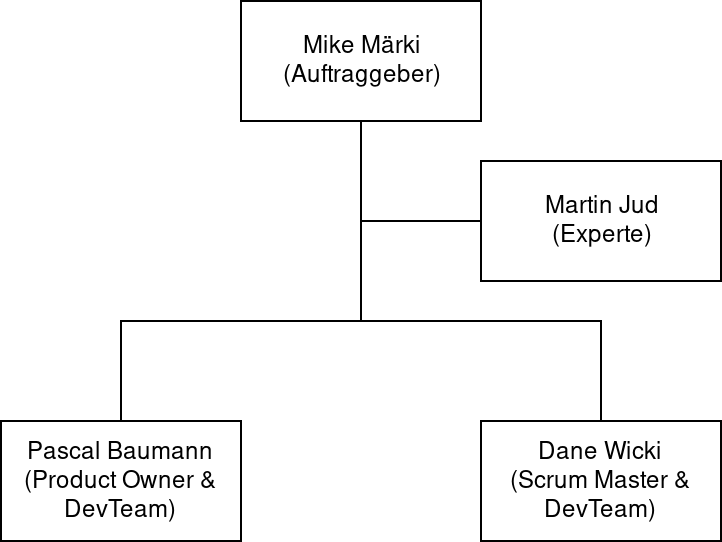
\includegraphics[keepaspectratio, width=0.6\textwidth]{OrganigrammBDA_BAWI.png}
\end{figure}

\subsection{Rollen im Team}
Hier werden die Hauptverantwortlichkeiten des Jeweiligen Teammitgliedes niedergeschrieben. Dies bedeutet nicht, dass dieses jeweilige Mitglied für diese Funktion, Tätigkeit oder Aufgabe alleine zuständig war, sondern lediglich, dass die Entscheidungsgewalt, sowie die Verantwortung bei diesem liegt.

\begin{tabularx}{\textwidth}{|l|X|}
	\hline
	\textbf{Teammitglied} & \textbf{Funktion/Tätigkeit/Aufgaben} \\
	\hline
	Pascal Baumann & Stand der Forschung \\
		& Konzept 2 (Verhinderung des Deplatzieren eines Exemplars) \\
		& Machbarkeitstudie Recherche \\
		& Support Dokumentationssoftware \\
		& Grobplanung \\
		& Risikoanalyse \\
		& CI/CD Dokumentation \\
	\hline
	Dane Wicki & Konzept 1 (Auffindung eines deplatzierten Exemplars)\\
		& Requirements Engineering \\
		& Softwarearchitektur \\
		& Programming Language Advisor \\
		& CI/CD Software \\
		& RFID Hardwarebeschaffung und Verwaltung \\
		& Hardware Interface Specialist \\
		& Sitzungsprotokolle \\
		
	\hline
\end{tabularx}

\section{Rahmenplan}
\subsection{Meilensteine}
\label{ssec:Meilensteine}
Für das Projekt wurden vier Meilensteine definiert, welche jeweils im Vierwochenzyklus auftreten. Diese Meilensteine sind in Abbildung \ref{fig:Milestones} dargestellt.

\begin{figure}[htb]
	\centering
	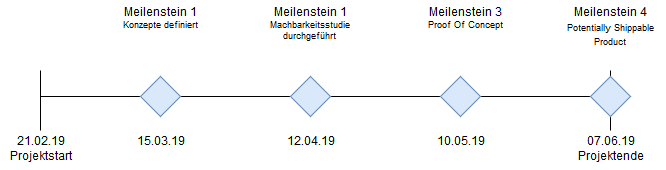
\includegraphics[keepaspectratio,width=0.8\linewidth]{Milestones.png}
	\caption{Die für das Projekt definierten Meilensteine}
	\label{fig:Milestones}
\end{figure}

\subsection{Grobplan}

Aus den im Kapitel \ref{ssec:Meilensteine} definierten Meilensteine wurden acht Sprints von zwei Wochen abgeleitet. In diesen werden sowohl die Artefakte wie Projektdokumentation, Machbarkeitsstudien und Systemspezifikation, wie auch das Produkt entwickelt. Der grobe Rahmenplan ist in Abbildung \ref{fig:Rahmenplan_1} dargestellt.

\begin{figure}[htb]
	\centering
	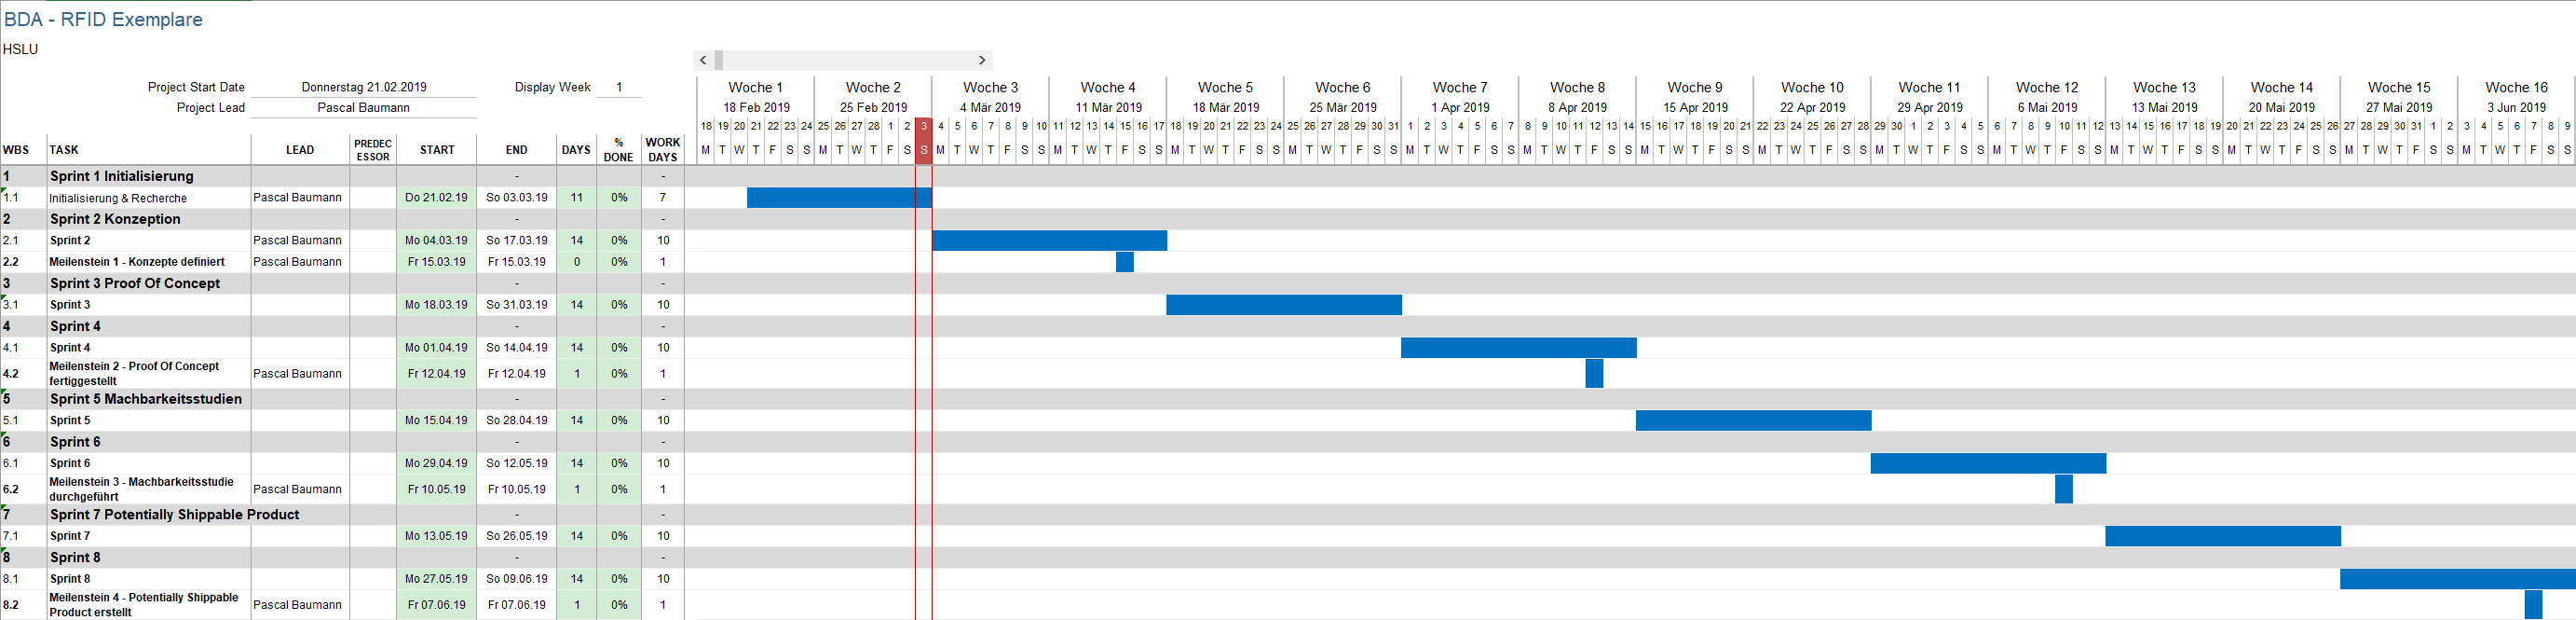
\includegraphics[keepaspectratio,width=\linewidth]{Grobplan.png}
	\caption{Übersicht der Sprints im Rahmenplan}
	\label{fig:Rahmenplan_1}
\end{figure}

\section{Beschreibung der Sprints}

\subsection{Sprint 01}
Das Sprintziel des ersten Sprints war der Wissensaufbau bezüglich RFID und wie eine Machbarkeitsstudie durchgeführt werden muss.

Im Vorfeld erstellte Herr Baumann einen Grobplan, eine erste Risikoanalyse und bereitete die Struktur der Dokumentation vor. Das Team bereitete sich auf das Meeting vor, indem es sich intensiv mit der Aufgabenstellung auseinandersetzte und bereits technische Überlegungen anstellte. Ungewissheiten wurden dabei gleich als Fragen für den Kunden erarbeitet, zudem wurde ein grober Zeitplan erarbeiteten. Das Kickoff-Meeting wurde aufgezeichnet und von Herrn Wicki in ein Protokoll transkribiert. Danach begann Herr Wicki mit der Anforderungsanalyse und Aktualisierte die Aufgabenstellung mit den gewonnenen Erkenntnissen. Herr Baumann las sich in die Erstellung einer Machbarkeitsstudie ein und erarbeitete ein Merkblatt für das Team. Das Projektteam las sich in die RFID Protokolle ein und erstellte einen ersten Entwurf der Stand der Technik, Herr Baumann konzentrierte sich dabei mehr um die technischen und theoretischen Voraussetzungen, während Herr Wicki über Referenzimplementationen Recherchen anstellte. Unter anderem wurde dabei der Hersteller der aktuell in der Speicherbibliothek eingesetzten Geräte ermittelt. Insgesamt verlief dieser Sprint aufgrund der Vorbereitungsarbeiten sehr flüssig und gab dem Projekt von Anfang an einen Aufwind.

Angetroffene Probleme waren die Unbekannten im Bezug auf das Projekt und wie eine Machbarkeitsstudie durchgeführt werden soll. Durch die Planung konnten diese Probleme jedoch angegangen werden. Es wurde ein Merkblatt zur Durchführung einer Machbarkeitsstudie erstellt und dem Team präsentiert und durch die Recherchen konnten technische Limitationen von HF RFID identifiziert werden.

\subsection{Sprint 02}
Das Sprintziel des zweiten Sprints waren die Erarbeitung und Spezifikation von zwei Konzepten.

Daher wurden die Erkenntnisse aus der Recherchephase umgesetzt. Im Speziellen erhielt Herr Baumann den Auftrag eine Struktur für die Machbarkeitsstudie zu erarbeiten und dem Team zur Verfügung zu stellen, er sollte auch die bestehende Projektdokumentation den Vorgaben der Hochschule für studentische Arbeiten anpassen. Nach einer Ideenfindung einigte man sich im Team zwei Konzeptideen genauer auszuarbeiten. Herr Baumann konzentrierte sich dabei auf eine stationäre Lösung beim Rüstplatz, während Herr Wicki ein Konzept für die automatische Suche im Lager erarbeitete. Beide Lösungskonzepte wurden anschliessend im Team präsentiert. Daraus ergab sich die Notwendigkeit Hersteller anzufragen, welche Lösungen mit einer Reichweite von mindesten 90cm anbieten. Herr Wicki fasste diesen Auftrag und ermittelte zwei passende, in Europa ansässige Hersteller. Die zwei erarbeiteten Konzepte wurden in einer Sitzung dem Kunden präsentiert und abgenommen. Insgesamt verlief dieser Sprint gut und es konnten Fortschritte in alle Richtungen (Projekt, Dokumentation, Kundendeliverables) verzeichnet werden.

Probleme verursachten vor allem die Ideenfindung für die Konzepte, insbesondere die Idee einer Suchbox stellte sich als schwierig an, da die Recherchen ergaben, dass die maximale Lesereichweite von HF RFID Lesern bei knapp einem Meter lag. Das Problem wurde durch eine gemeinsame Ideenfindung und Ausarbeitung der Konzeptidee gelöst. Danach wurden die Konzepte erfolgreich spezifiziert, dokumentiert und ausgearbeitet. Das Sprintziel konnte somit erfolgreich erreicht werden und die interne Zusammenarbeit verlief effizient und sehr zufriedenstellend.

\subsection{Sprint 03}
Das Sprintziel des dritten Sprints war die Akquisition und insbesondere Erhalt, eines HF RFID-Lesegeräts mit mindestens zwei Antennen.

Aus der Meilensteinsitzung wurde klar, dass die Kosten für die ermittelten Geräte für Testzwecke und Prototypisierung zu hoch sind, und die nötigen Geldmittel weder vom Kunden noch vonseiten der Hochschule zur Verfügung stehen. Als Sprintziel wurde die Akquisition von Versuchsgeräten definiert. Das Projektteam versuchte noch einmal Testgeräte bei Bildungseinrichtungen, Hochschulen und Herstellern zu erhalten. Herr Baumann kontaktierte dafür Gewerbeschulen in der Zentralschweiz und Kompetenzzentren für RFID an den Hochschulen Luzern und Winterthur. Herr Wicki kontaktierte Vertreiber von HF RFID Lösungen, ob diese Leihgeräte zur Verfügung stellen könnten. Weiter wurden auch die Budgetvorstellungen der Hochschule dem Projektteam mitgeteilt. Weiter wurde vom Projektteam das Protokoll für die Meilensteinsitzung erarbeitet. Die Herausforderung in diesem Sprint waren vor allem die Schwierigkeiten im Bezug auf die Versuchsgeräte, insbesondere der Erhalt der Vielzahl von Absagen.

In diesem Sprint stellten sich vor allem Budgetprobleme vonseiten des Kunden und der Hochschule. Gelöst werden konnte diese nur durch Eigeninvestitionen und günstigeren Produkten aus China. Da die Produkte nur bestellt, aber nicht bei uns eingetroffen waren, konnte das Sprintziel nicht erreicht werden. Positiv war, dass durch die agile Projektmethode auf das Problem reagiert werden konnte, und dieser und subsequente Sprints umgeplant werden konnte.

\subsection{Sprint 04}
Das Sprintziel des vierten Sprints war die Fertigstellung, das heisst Implementation aller kritischen Komponenten, sodass die Versuche durchgeführt werden konnten, des Testframeworks bis auf Treiber und die Definition der Versuche.

In diesem Sprint wurden die erarbeiteten Konzepte noch einmal kritisch begutachtet, harmonisiert und für die Machbarkeitsstudie finalisiert. Alle Versuche Leihgaben zu erhalten scheiterten jedoch. Vonseiten der Hersteller erhielt man zwar Rabatte. Die Preise für die Geräte waren jedoch immer noch ein Vielfaches von dem, was die Hochschule bereit war für eine BDA zur Verfügung zu stellen. Das Team entschied sich, um reelle Aussagen in der Machbarkeitsstudie machen zu können, auf eigene Kosten bei einem Hersteller in China zu bestellen. Diese Geräte trafen dann auf Ende Sprint beim Team ein. Um nicht zu viel Zeit zu verlieren, entschied das Team sich, Versuche genau zu spezifizieren, Versuchsmaterialien zu beschaffen und ein Testframework zu definieren. Dieses war vor allem nötig um im Millisekundenbereich Gerätefunktionen zu testen, was von Hand gar nicht oder nur begrenzt möglich ist. Am Ende dieses Sprints stand die Zwischenpräsentation des Projekts an. Diese wurde von beiden Teammitgliedern erarbeitet, antrainiert und dem Betreuer und Experten präsentiert. Die Herausforderung dieses Sprints war der Motivationsdämpfer aufgrund der Schwierigkeiten und Ungewissheit im Bezug auf die Versuchsgeräte und dem weiteren Verlauf des Projekts.

Der Sprint war durch eine Vielzahl von Problemen geplagt. Zum einen war dies die späte Ankunft der Testgeräte auf das Ende des Sprints, zum zweiten die Verzögerung des Abschlusses des letzten Sprints und dadurch eine Verkürzung dieses Sprints und zum Schluss fehlende Ressourcen durch die Arbeitstätigkeit eines Teammitglieds. All dies führte dazu, dass das Sprintziel nicht erreicht wurde. Um einen solchen Sprint nicht noch einmal erleben zu müssen, wurde am Anfang des nächsten Sprints eine detaillierte Retrospektive durchgeführt und Massnahmen definiert. Das Resultat war eine klar fixierte Zeit für ein wöchentlich stattfindendes, telefonisches Meeting und Austausch zwischen den Teammitgliedern.

\subsection{Sprint 05}
Das Ziel des fünften Sprints war die Durchführung und Dokumentation der im letzten Sprint definierten Versuche.

Bevor die Versuche durchgeführt werden konnten, musste ein Treiber für die Geräte entwickelt werden. Herr Wicki fragte diesbezüglich beim Händler die Spezifikation der Schnittstelle an und entwickelte einen Treiber. Herr Baumann kümmerte sich um die Benutzerschnittstelle und das Einpflegen der Versuchsdefinitionen. Weiter begann die Arbeit an der Machbarkeitsstudie, wobei Herr Baumann das Projektumfeld der Machbarkeitsstudie und Herr Wicki die Beschreibung des Projektes im Kontext der Machbarkeitsstudie in Angriff nahm.

Das angetroffene Problem dieses Sprints war, dass die Spezifikation des Gerätetreibers weniger gut als erhofft war. Insbesondere muss die DLL des Händlers verwendet werden, welche nur durch eine 32bit Applikation aufgerufen werden kann, und dazu keine Betriebssystemunabhängigkeit zulässt. Gelöst wurde dies, indem Windows und JNI/JNA verwendet wurde. Positiv war, dass das Sprintziel erfolgreich erreicht und die angetroffenen Probleme behoben werden konnten.

\subsection{Sprint 06}
Das Sprintziel dieses Sprints lag in der Fertigstellung der Machbarkeitsstudie.

Bedingt durch das Sprintziel wurden die Kapitel der Machbarkeitsstudie in jeweils 5-13h Arbeitspakete unterteilt und diese anschliessend unter beiden projektdurchführenden Personen aufgeteilt. So schrieb Herr Wicki die Kapitel Investitions- und Betriebskosten, Beschreibung des Projekts, technische Aspekte und das Finding Summary wie auch das Abstract. Herr Baumann schrieb seinerseits die Kapitel Projektumfeld, Entwicklungsplan und markttechnische Aspekte.
Gegen Ende des Sprints gab es zudem noch eine Meilensteinsitzung, bei welcher die erarbeiteten Artefakte, namentlich die Machbarkeitsstudie wie auch die Ergebnisse der Tests, an Herr Märki präsentiert und abgegeben wurde. Bei dieser Meilensteinsitzung wurden noch die Anforderungen für die kommende Entwicklung des MVPs besprochen, da einige Anforderungen noch zu generisch beschrieben waren. Bei dieser Absprache konnte schliesslich noch ein Missverständnis identifiziert werden, bei welchem das Team davon ausging, dass die Tag-ID in der Datenbank gespeichert ist, jedoch sei nicht der Fall ist und nur die Buch-ID, welche auch als Barcode auf dem Buch ist, in der Datenbank zu finden ist. Anschliessend wurden alle Anforderungen nochmals durchgegangen und auf deren Erfüllung überprüft.

Die Probleme während diesem Sprint hielten sich in Grenzen. So gab es lediglich das Problem, dass keiner der beiden Studierenden mit dem Schreiben einer Machbarkeitsstudie stark vertraut war und es dadurch zu der Situation kam, bei welcher eine Tabelle dupliziert im Dokument anzutreffen war. In einer kurzen Besprechung konnte jedoch gemeinsam der passende Absatz im Dokument gefunden werden für diese Tabelle, sodass diese nur noch einmal vorhanden ist.

\subsection{Sprint 07}
Das Sprintziel dieses Sprints lag in der Fertigstellung der Referenzimplementation.

 Dazu wurde die Implementation der Applikation in mehrere Arbeitspakete unterteilt und im Team aufgeteilt. Als Erstes wurde in einer gemeinsamen Sitzung eine Architekturidee entworfen. Anschliessend mussten einige Arbeitspakte neu hinzugefügt werden, da mit der Architekturidee neue Aufgaben entstanden. Zudem musste ein Arbeitspaket entnommen werden, dies aus dem Grund, dass während der Sitzung die Entscheidung getroffen wurde, dass die von Herr Märki nicht priorisierte Anforderung zur Einbindung der Datenbank aus Zeitgründen nicht implementiert wird. Parallel zur Entwicklung der Referenzimplementation wurde an der Dokumentation gearbeitet und diese verbessert. Weiter wurde während diesem Sprint auch das WebAbstract erstellt.

 Während diesem Sprint stiess das Projektteam auf verschiedene Probleme, welche gelöst werden mussten. So wurden bei der Einrichtung der CI/CD Pipeline der Referenzimplementation die in Kotlin geschriebenen Unit-Tests nicht ausgeführt. Dieses Problem entstand, da sich das Team auf die Verwendung von JUnit5 einigte und das build.gradle Skript für diese Version von JUnit noch zusätzliche Konfigurationen benötigt. Weiter wurde versucht die Applikation mit Java12 zu betreiben. Es musste jedoch wieder auf Java 8 zurückgegriffen werden, das für Java 12 keine 32Bit Version gefunden werden konnte und dies eine Voraussetzung für den RFID Hardwaretreiber ist. In der Hälfe des Sprints wollte das Team die CI/CD Pipeline ausbauen, sodass eine .jar-Datei erstellt wurde, welches alle Abhängigkeiten enthält (auch fatJar genannt). Dabei stiess das Team auf das Problem, dass Abhängigkeiten zu anderen Bibliotheken nicht in die erstellte .jar-Datei eingebettet wurden. Es stellte sich heraus, dass es mit der Konfiguration im build.gradle Skript gelöst werden konnte, indem die Abhängigkeiten mit dem Schlüsselwort "compile" anstelle "implementation" in der Konfiguration eingebunden werden. Ein weiteres Problem war die Erstellung eines PDF/A Dokumentes, welches direkt durch das Buildtool PdfLaTeX generiert werden soll. Dazu wurden vom Team verschiedene Latex Packages ausprobiert, bis herausgefunden wurde, dass das Latex Package "pdfx" in Kombination mit einem .xmpdata-Datei ein PDF/A Dokument erstellt, mit den korrekten, in der .xmpdata-Datei definierten Metadaten.

\subsection{Sprint 08}
Das Ziel dieses Sprints lag in der Fertigstellung und Abgabe der Dokumentation.
Um dieses Ziel zu erreichen wurde, während der Sprintplanung, die Dokumentation auf fehlende Inhalte überprüft und für diese jeweils ein Arbeitspaket erstellt. Zu Beginn des Sprints wurde die Referenzimplementation noch bei der Speicherbibliothek vor Ort getestet. Dabei wurden noch kleinere Softwareanpassungen vorgenommen, um die Stabilität der Referenzimplementation zu verbessern und die Ausgabegeschwindigkeit zu erhöhen. Anschliessend folgte noch ein kurzer Austausch mit Herr Märki, bei welchem kleinere Unstimmigkeiten in der Machbarkeitsstudie besprochen wurden. Diese Besprechung führte dazu, dass noch ein Arbeitspaket für die Korrektur dieser Unstimmigkeiten erstellt wurde. Nach dem Test vor Ort der Referenzimplementation, konnte noch ein Designfehler in dieser gefunden und korrigiert werden. Dieser Fehler hatte jedoch keine Auswirkungen auf die Ausführung, sehr wohl jedoch auf die Lesbarkeit. 
Weiter konnte im Verlauf des Sprints noch ein konstruktives Feedback von Herr Jud, bezüglich dem inhaltlichen Aufbau der Dokumentation, abgeholt werden. Dieses Feedback führte zu einem Replanning, bei welchem neue Arbeitspakete erstellt wurden, welche die von Herr Jud kritisierten Punkte verbesserten. Gegen Ende des Sprints konnte die Dokumentation in einen finalisierten Zustand gebracht werden, in welcher die Dokumentation schliesslich abgegeben wurde.

Während dem Sprint traten keine gravierenden Probleme auf.
Es musste jedoch zweimal auf ein Feedback eingegangen werden. Welche zu einem kleineren Replanning führten. Dies konnte jedoch durch die gute Zusammenarbeit erfolgreich durchgeführt werden.
\newpage

\section{Tools}
\label{sec:Tools}

\subsection{Versions Kontrolle}
\begin{table}[h!]
	\begin{tabular}{p{0.5\textwidth} p{0.5\textwidth}}
		\hline
		\textbf{Tool} & \textbf{Version} \\
		\hline
		GitKraken & 4.2.2 \\
		\hline
		git & 2.21.0 \\
		\hline
		GitHub & GitHub.com \\
		\hline
	\end{tabular}
	\caption{Verwendete Versionen der Versionierungssysteme}
\end{table}

\subsection{Dokumentation}
\begin{table}[h!]
	\begin{tabular}{p{0.5\textwidth} p{0.5\textwidth}}
		\hline
		\textbf{Tool} & \textbf{Version} \\
		\hline
		TeX Live & 2018 \\
		\hline
		MiKTex & 2.9.6637 \\
		\hline
		Mendeley Desktop & 1.19.2 \\
		\hline
		MS Excel & 16.0.11231.20164 \\
		\hline
	\end{tabular}
	\caption{Verwendete Versionen der Hilfsmittel für die Dokumentation}
\end{table}


\subsection{Repositories \& Buildtools}
\begin{table}[h!]
	\begin{tabular}{p{0.5\textwidth} p{0.5\textwidth}}
		\hline
		\textbf{Name} & \textbf{URL} \\
		\hline
		Dokumentation & \url{https://github.com/HSLU-BaumannWicki/BDA_FS19-Dokumentation} \\
		\hline	
		Travis CI &  \url{https://travis-ci.org/HSLU-BaumannWicki/BDA_FS19-Dokumentation} \\
		\hline
	\end{tabular}
	\caption{Verwendete Repositories}
\end{table}

\subsection{Übrige}
\begin{table}[h!]
	\begin{tabular}{p{0.5\textwidth} p{0.5\textwidth}}
		\hline
		\textbf{Tool} & \textbf{Verwendung} \\
		\hline
		Trello & Aufgabenverwaltung \\
		\hline
		Scrum Poker Online & Storypoints Estimation\\
		\hline
		WhatsApp & Kommunikation im Team \\
		\hline
		OneDrive Online & Dokumentenspeicher \\
		\hline	
	\end{tabular}
	\caption{Übrige Hilfsmittel}
\end{table}

\clearpage

\section{Risikomanagement}

Es werden mögliche Risiken, welche während dem Projekt auftreten können aufgezählt. Diese werden auf Eintrittswahrscheinlichkeit und Schadensmass eingeschätzt, danach wird entschieden, welche Massnahmen getroffen werden können, und was deren Auswirkungen sind.

\subsection{Definitionen}
\label{sssec:Def}
\vspace{1em}
\noindent
Eintrittswahrscheinlichkeit:

\vspace{1em}
\noindent
\begin{tabularx}{\textwidth}{|l|l|X|}
	\hline
	\textbf{Stufe} & \textbf{Bezeichnung} & \textbf{Beschreibung} \\
	\hline
	1 & unvorstellbar & Möglich aber eher unwahrscheinlich. Tritt nie oder einmal in 16 Wochen auf \\
	\hline
	2 & unwahrscheinlich & Kann in 16 Wochen kein oder ein Mal eintreten\\
	\hline
	3 & vorstellbar & Kann in 16 Wochen ein bis zwei Mal eintreten \\
	\hline
	4 & wahrscheinlich & Kann in 16 Wochen bis zu drei Mal eintreten \\
	\hline
	5 & häufig & Kann in 16 Wochen sieben Mal eintreten\\
	\hline
\end{tabularx}

\vspace{1em}
\noindent
Schadensausmass:

\vspace{1em}
\noindent
\begin{tabularx}{\textwidth}{|l|l|X|}
	\hline
	\textbf{Stufe} & \textbf{Bezeichnung} & \textbf{Beschreibung} \\
	\hline
	1 & unwesentlich & Die Aufgabenerfüllung wird höchstens geringfügig beeinträchtigt, finanzieller Schaden ist im Rahmen des Projekts nicht beeinflussend. Personenschäden treten nicht auf. \\
	\hline
	2 & geringfügig & Wahrnehmbare Gefährdung / Einfluss auf das Projekt. Personenschäden treten nicht auf. \\
	\hline
	3 & mittelmässig & Wahrnehmbare Gefährdung / Einfluss auf das Projekt. Verzögerungen zur Folge. Finanzieller Schaden strapaziert das Projektbudget. Personenschäden treten nicht auf. \\
	\hline
	4 & kritisch & Starke Gefährdung des Projekts. Extreme Verzögerungen zur Folge. Finanzieller Schaden übersteigt das Projektbudget. Personenschäden treten geringfügig auf.\\
	\hline
	5 & katastrophal & Projektabbruch zur Folge. Finanzieller Schaden kann zum Projektstopp führen. Verletzung der Persönlichkeitsrechte. \\
	\hline
\end{tabularx}

\newpage

\subsection{Risikokatalog}
\label{sssec:Risikokatalog}
Legende:
\begin{itemize}
	\item \textbf{S}chadensausmass bei Eintreffen des Risikos
	\item \textbf{W}ahrscheinlichkeit das Risiko eintrifft
	\item \textbf{K}ategorie: \textbf{T}echnisches oder \textbf{P}rojektbezogenes Risiko
	\item \textbf{A}uswirkung auf das Projekt. Produkt aus S und W
\end{itemize}

\vspace{1em}
\noindent
\begin{table}[htb]
	\begin{tabularx}{\textwidth}{|l|X|l|l|l||l|}
		\hline
		\textbf{Nr.} & \textbf{Beschreibung / Risiko} & \textbf{K} & \textbf{S} & \textbf{W} & \textbf{A} \\
		\hline
		1 & Meilensteine werden nicht erreicht & P & 4 & 2 & 8 \\
		\hline
		2 & Teammitglied fällt aus & P & 4 & 1 & 4 \\
		\hline
		3 & Fehlkommunikation im Team & P & 4 & 1 & 4 \\
		\hline
		4 & Produkt entspricht nicht den Kundenanforderungen & P & 5 & 2 & 10 \\
		\hline
		5 & Umsetzung des Produkts technisch nicht möglich & T & 3 & 3 & 9 \\
		\hline
		6 & Datenverlust & T & 5 & 2 & 10 \\
		\hline
		7 & Lieferschwierigkeiten von Teilen & P & 3 & 3 & 9 \\
		\hline
		8 & Kosten übersteigen Budgetvorstellung des Kunden & P & 3 & 2 & 6\\
		\hline
		9 & Kosten übersteigen Budgetvorstellung der Hochschule & P & 3 & 3 & 9\\
		\hline
	\end{tabularx}
	\caption{Die im Projekt identifizierten Risiken}
	\label{tbl:Risks}
\end{table}

\vspace{1em}

\begin{figure}[htb]
	\centering
	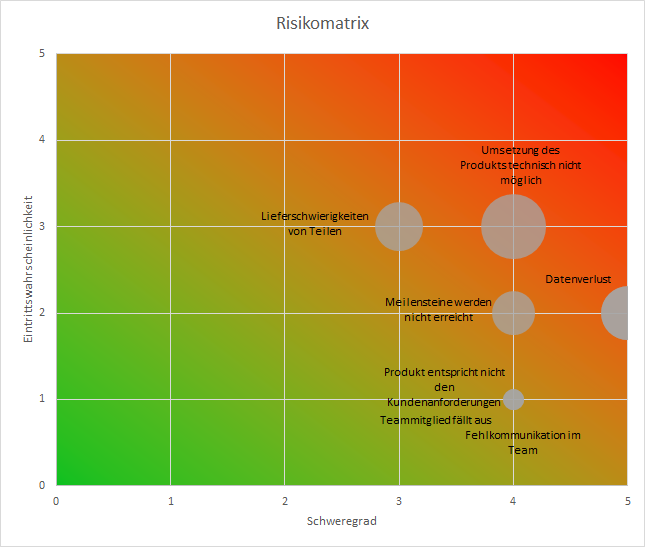
\includegraphics[keepaspectratio, width=0.6\textwidth]{Risks_before.png}
	\caption{Auswirkungen der in Tabelle \ref{tbl:Risks} identifizierten Risiken}
\end{figure}

\newpage

\subsubsection{Massnahmen}

\begin{table}[htb]
	\begin{tabularx}{\textwidth}{|l|X|}
		\hline
		\textbf{Nr.} & \textbf{Beschreibung Massnahme} \\
		\hline
		1 & Meilensteine werden in zwei Zweiwöchigen Sprints absolviert. Die Tasks pro Sprint werden weiter detailliert heruntergebrochen. So sollen die Arbeiten sowohl auf Makro- wie Mikrosicht eingeplant werden. \\
		\hline
		2 & Arbeiten werden so strukturiert und dokumentiert, dass das zweite Mitglied diese auch übernehmen kann. Es werden Spezialisierungen der Teammitglieder insoweit verhindert, dass Wissenslücken minimiert werden. Recherchen sollen Zusammenfassungen und Merkblätter über die gewonnenen Erkenntnisse als Resultat haben.\\
		\hline
		3 & Der Kontakt wird von beiden Teammitgliedern sowohl horizontal im Team wie auch vertikal zu den Stakeholdern aktiv gesucht. Es werden den Arbeiten auch teambildende Aktivitäten zusammen absolviert.\\
		\hline
		4 & Der Kunde muss den Fortschritt alle vier Wochen in einer Sitzung kontrollieren, avisieren und, wenn nötig, Anpassungen fordern.\\
		\hline
		5 & Es soll während den Recherchen schon im Hinblick auf die technische Umsetzung acht gegeben werden.\\
		\hline
		6 & Sowohl produzierten Artefakte, wie auch aktuelle getätigte Arbeiten werden auf auswärtige Plattformen ausgelagert.\\
		\hline
		7 & Teile werden bei Bedarf sofort bestellt, es werden inländische, etablierte Lieferanten, vor evtl. günstigeren Ausländischen vorgezogen.\\
		\hline
		8 & Lösungskonzept wird in der erarbeiteten Form verworfen und durch günstigere Komponenten ersetzt.\\
		\hline
		9 & Es werden alternative Sponsoren von Geldmittel gesucht.\\
		\hline
	\end{tabularx}
	\caption{Massnahmen um Effekte oder Eintrittswahrscheinlichkeit zu reduzieren}
\end{table}

\vspace{1em}

\begin{table}[htb]
	\begin{tabularx}{\textwidth}{|l|X|l|l|l||l|}
		\hline
		\textbf{Nr.} & \textbf{Beschreibung / Risiko} & \textbf{K} & \textbf{S} & \textbf{W} & \textbf{A} \\
		\hline
		1 & Meilensteine werden nicht erreicht & P & 4 & 1 & 4 \\
		\hline
		2 & Teammitglied fällt aus & P & 3 & 1 & 3 \\
		\hline
		3 & Fehlkommunikation im Team & P & 4 & 1 & 4 \\
		\hline
		4 & Produkt entspricht nicht den Kundenanforderungen & P & 5 & 1 & 5 \\
		\hline
		5 & Umsetzung des Produkts technisch nicht möglich & T & 4 & 3 & 12 \\
		\hline
		6 & Datenverlust & T & 5 & 1 & 5 \\
		\hline
		7 & Lieferschwierigkeiten von Teilen & P & 3 & 2 & 6 \\
		\hline
		8 & Kosten übersteigen Budgetvorstellung des Kunden & P & 3 & 1 & 3\\
		\hline
		9 & Kosten übersteigen Budgetvorstellung der Hochschule & P & 3 & 2 & 6\\
		\hline
	\end{tabularx}
	\caption{Neueinschätzung der Risiken nach Einführung der Massnahmen}
	\label{tbl:Massnahmen}
\end{table}

\vspace{1em}

\begin{figure}[htb]
	\centering
	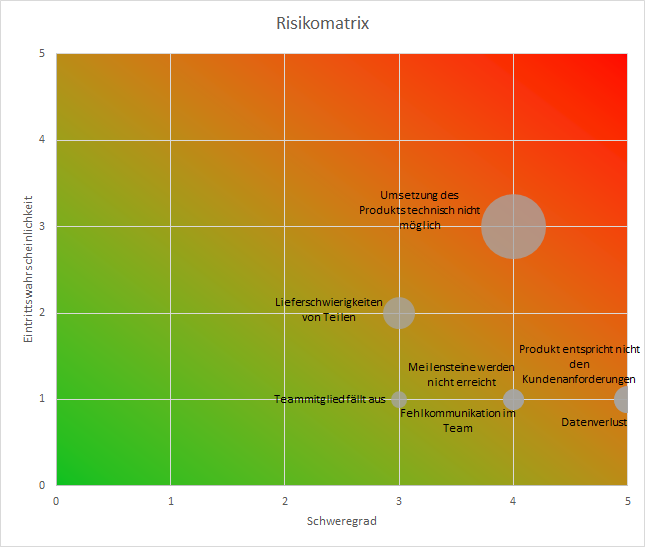
\includegraphics[keepaspectratio, width=0.6\textwidth]{Risks_after.png}
	\caption{Auswirkungen der Risiken nach den in Tabelle \ref{tbl:Massnahmen} vorgeschlagenen Massnahmen}
\end{figure}
